\pdfoutput=1
\documentclass[pra,twocolumn,showpacs,amsmath,amssymb]{revtex4-1}

\usepackage{graphicx}%Include figure files
\usepackage{dcolumn}%Align table columns on decimal point
\usepackage{bm}% bold math
\usepackage{subcaption}


%\nofiles

\begin{document}

\newcommand{\trel}{$\tau_A / \tau_B$}

\title{Project 1: Modelling Radioactive Decay}


\author{John Russo}
\affiliation{Department of Physics and Astronomy, University
of Delaware, Newark, DE 19716-2570, USA}

\begin{abstract}
Abstract goes here.
\end{abstract}

\pacs{}


\maketitle





\section{Introduction} \label{sec:intro}

Modelling radioactive decay involves only a simple numerical solution to a
differential equation. However, it is a useful demonstration of basic numerical
solving techniques, with a wide range of applications.
Radioactive decay is a stochastic process where a nucleus breaks down, releasing
energy, matter, or both, depending on the type of decay.
Radioactive decay is a process studied for applications from nuclear weapons to
carbon dating, where understanding decay rates of isotopes can yield information
about age of a sample.





\section{Method}

\subsection{Part I - Decay}


In Part I of this project, numerical solutions are plotted for the case of two
populations of nuclei, $A$ and $B$. $A$ nuclei decay into $B$ nuclei. $B$
nuclei also decay.

Decay of these populations is governed by the following first-order coupled
differential equations

\begin{align}
  \frac{d N_A}{dt} &= -\frac{N_A}{\tau_A} \\
  \frac{d N_B}{dt} &= \frac{N_A}{\tau_A} - \frac{N_B}{\tau_B}
\end{align}

where $N_A$ and $N_B$ are the $A$ and $B$ nucleus populations, and $\tau_A$ and
$\tau_B$ are the respective e-folding times of the nuclei.

These equations can be normalized to

\begin{align}
  \frac{d \bar N_A}{d \bar t} &= - \bar N_A \label{eq:decay_A_norm}\\
  \frac{d \bar N_B}{d \bar t} &= \bar N_A - \frac{\tau_A}{\tau_B} \label{eq:decay_B_norm}\bar N_B
\end{align}

where bars indicate the normalized variables.

Numerical solutions are obtained by Euler stepping with a fixed time interval $dt$.

\subsection{Part II - Resonance}

In Part II a system is analyzed where $B$ nuclei decay back into $A$ nuclei.
This system is described by

\begin{align}
  \frac{d N_A}{dt} &= \frac{N_B}{2 \tau} - \frac{N_A}{\tau} \\
  \frac{d N_B}{dt} &= \frac{N_A}{\tau} - \frac{N_B}{2 \tau}
\end{align}

which are normalized to

\begin{align}
  \frac{d \bar N_A}{d \bar t} &= -  \bar N_A + \frac{1}{2} \bar N_B \label{eq:res_A_norm} \\
  \frac{d \bar N_B}{d \bar t} &=  \bar N_A - \frac{1}{2} \bar N_B \label{eq:res_B_norm}.
\end{align}





\section{Results}

\subsection{Part I}

Varying the parameter \trel~demonstrates its affect on the
system's transient and steady state behavior.

Examining Eqs.~\ref{eq:decay_A_norm} and \ref{eq:decay_B_norm}, the ratio
 \trel~only affects the decay of the $B$ population, whereas the $A$
 population's decay is affected solely by the size of the $A$ population.
 %
This is consistent with Figs.~\ref{fig:tau_gt_1}-\ref{fig:tau_lt_1}, which show
the $A$ population decaying at a constant rate regardless of the value of \trel.
These plots also show that decreasing \trel~decreases the slope of $N_B$,
in other words slowing the decay rate of the $B$ population.

Physically, this means that if the $B$ population has a longer e-folding time,
meaning it is more stable than the $A$ population, then the $B$ population decays
more slowly than the $A$ population.

\begin{figure}
  \begin{subfigure}[t]{.7\linewidth}
    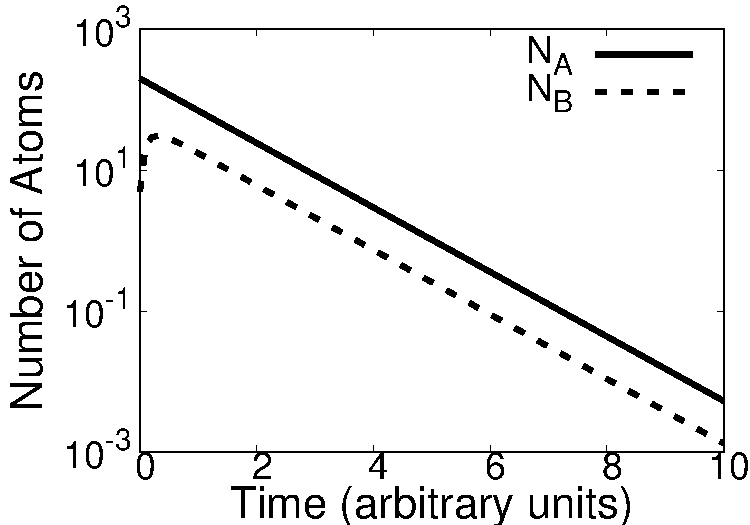
\includegraphics[width=\linewidth]{t_gt_1.pdf}
    \caption{$\tau_A / \tau_B=5$}
    \label{fig:tau_gt_1}
  \end{subfigure}
~
  \begin{subfigure}[t]{.7\linewidth}
    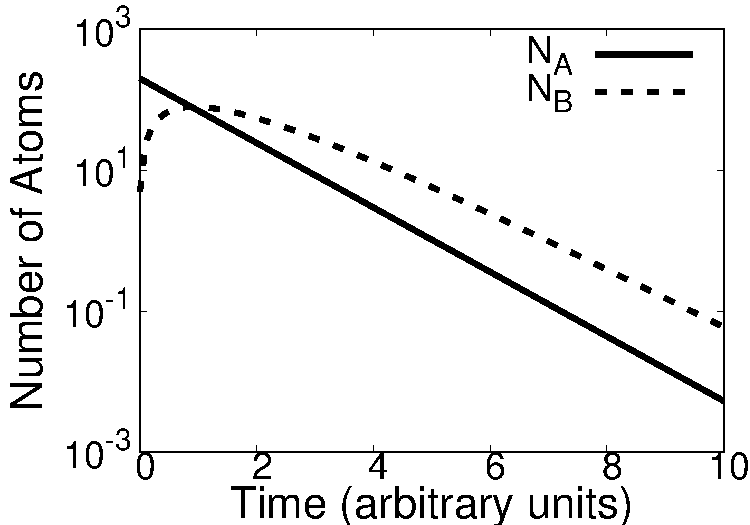
\includegraphics[width=\linewidth]{t_eq_1.pdf}
    \caption{$\tau_A / \tau_B=1$}
    \label{fig:tau_eq_1}
  \end{subfigure}
~
  \begin{subfigure}[t]{.7\linewidth}
    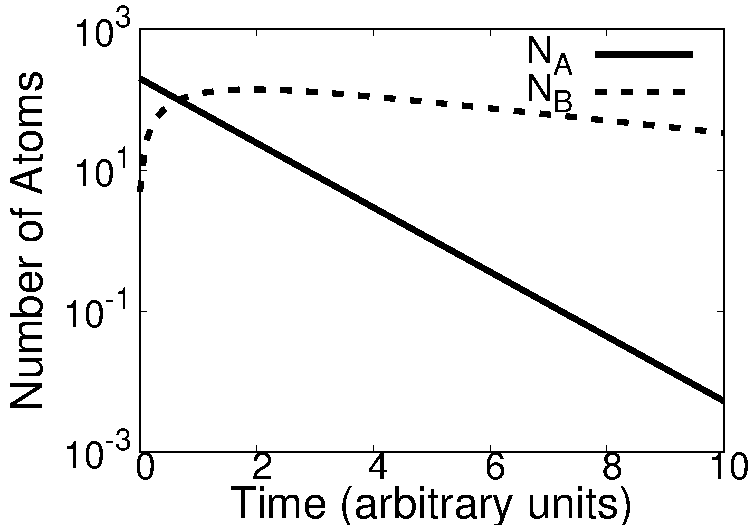
\includegraphics[width=\linewidth]{t_lt_1.pdf}
    \caption{$\tau_A / \tau_B=0.2$}
    \label{fig:tau_lt_1}
  \end{subfigure}

  \caption{$A$ and $B$ nucleus populations for various values of \trel.
  All figures generated with $dt=0.1$. Semilog axes are used to highlight the
  exponential decay of the populations.}
\end{figure}

\subsubsection{Stability Analysis}

It is also interesting to analyze the stability of this numerial analysis for
different timestep lengths $dt$. In Figs.~\ref{fig:tau_gt_1}-\ref{fig:tau_lt_1},
$dt=0.1$ is much smaller than the characteristic timescales of the system defined
by $\tau_A$ and $\tau_B$. As a result, we observe smooth curves, without obvious
inaccuracies caused by numerical instability.

Additionally, we can note that the most rapid change in the system occurs between
roughly $t=0$ to $t=1$, after which $N_B$ settles into a constant
rate of exponential decay. So, while $dt$ is short enough to capture the dynamics
of this time, i.e. smaller than order $1$, we expect stable results.

We can verify this by varying the timestep length about 1. In

\begin{figure}[h!]
  \begin{subfigure}[t]{.8\linewidth}
    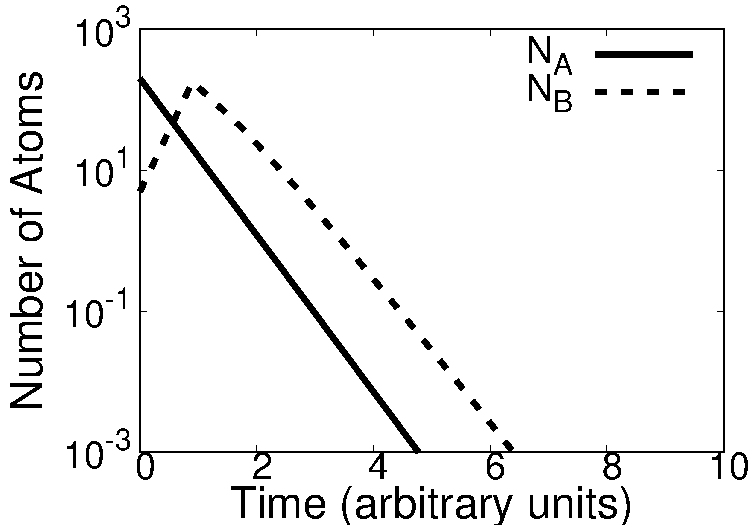
\includegraphics[width=\linewidth]{t_eq_1_unstable.pdf}
    \caption{ With $dt=0.9$, and so on the order of the initial change in the system, instability in the
    numerical analysis over the first step causes the system to decay much faster
    than it should.}
    \label{fig:tau_eq_1_unstable}
  \end{subfigure}

  \begin{subfigure}[t]{.8\linewidth}
    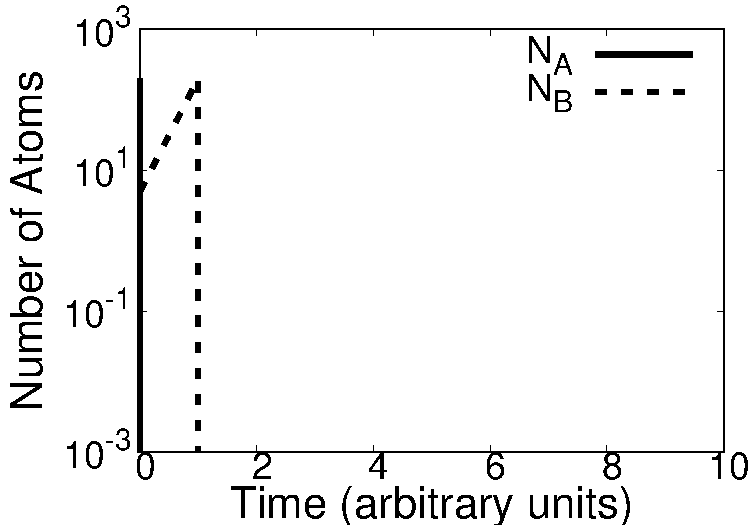
\includegraphics[width=\linewidth]{t_eq_1_vunstable.pdf}
    \caption{With $dt=1.0$,
    $dt$ is greater than the timescale over which change occurs,
    the instability is even more prominent, and the populations immediately go
    to 0.}
    \label{fig:tau_eq_1_vunstable}
  \end{subfigure}

  \caption{Plots of \trel~$ = 1$ as in Fig.~\ref{fig:tau_eq_1} with $dt$ varied
  to demonstrate instability in numerical analysis.}
\end{figure}


% I analyze three main cases for these populations based on the ratio
% $\tau_A / \tau_B$, which governs steady-state behavior of the system.
%
% \subsubsection{$\tau_A / \tau_B > 1$}
%
%
% \subsubsection{$\tau_A / \tau_B = 1$}
%
%
% \subsubsection{$\tau_A / \tau_B < 1$}


% For all results presented here, $N_A = 200, N_B = 5, \tau_A = 0.5$ and $\tau_B = 1.0$.
%
% \begin{figure}
%   \vspace{2ex}
%   \includegraphics[width=\linewidth]{../plot.pdf}
%   \caption{A and B particle populations, plotted against arbitrary time. Using
%   a shared linear axis, the large difference in population sizes makes
%   visualization of the data difficult.}
%   \label{fig:linplot}
% \end{figure}
%
% \begin{figure}
%   \vspace{2ex}
%   \includegraphics[width=\linewidth]{../logplot.pdf}
%   \caption{A and B particle populations, plotted against arbitrary time. The log
%   scale shows that though the populations decay at very different rates, the
%   linearity of each population's trajectory demonstrates exponential decay.}
%   \label{fig:logplot}
% \end{figure}
%
% In these figures, and particularly in Fig.~\ref{fig:linplot} one can observe the
% B particle population sharply peaking before beginning its decline. When the
% A population satisfies
% \begin{equation}
% \frac{N_A}{N_B} \geq \frac{\tau_A N_{B,0}}{\tau_B N_{A,0}}
% \end{equation}
% the growth rate of the B population is positive. For the given initial parameters,
% this means the B population should start declining when $N_A/N_B \geq 0.0125$.
%
% Observing the turnaround time here to be when the $N_B \approx 4000$,
% we can see in Fig.~\ref{fig:logplot} that at that time $N_A \approx 50$.

\subsection{Part II}


\section{Conclusions} \label{sec:conclusion}

\begin{thebibliography}{1}

\end{thebibliography}

\end{document}
